%%%%%%%%%%%%%%%%%%%%%%%%%%%%%%%%%%%%%%%%%
% Long Lined Cover Letter
% LaTeX Template
% Version 2.0 (September 17, 2021)
%
% This template originates from:
% https://www.LaTeXTemplates.com
%
% Authors: Fanchao Chen
% (chenfc@fudan.edu.cn)
%
% License:
% CC BY-NC-SA 4.0 (https://creativecommons.org/licenses/by-nc-sa/4.0/)
%
%%%%%%%%%%%%%%%%%%%%%%%%%%%%%%%%%%%%%%%%%

%----------------------------------------------------------------------------------------
%	PACKAGES AND OTHER DOCUMENT CONFIGURATIONS
%----------------------------------------------------------------------------------------

\documentclass{article}

\usepackage{charter} % Use the Charter font
\usepackage{ragged2e}
\usepackage{blindtext}
\usepackage{watermark}
\usepackage{tikz} 
\usepackage[
	a4paper, % Paper size
	top=1in, % Top margin
	bottom=1in, % Bottom margin
	left=1in, % Left margin
	right=1in, % Right margin
	%showframe % Uncomment to show frames around the margins for debugging purposes
]{geometry}

\setlength{\parindent}{0pt} % Paragraph indentation
\setlength{\parskip}{1em} % Vertical space between paragraphs

\usepackage{graphicx} % Required for including images

\usepackage{fancyhdr} % Required for customizing headers and footers

\fancypagestyle{firstpage}{%
	\fancyhf{} % Clear default headers/footers
	\renewcommand{\headrulewidth}{0pt} % No header rule
	\renewcommand{\footrulewidth}{1pt} % Footer rule thickness
}

\fancypagestyle{subsequentpages}{%
	\fancyhf{} % Clear default headers/footers
	\renewcommand{\headrulewidth}{1pt} % Header rule thickness
	\renewcommand{\footrulewidth}{1pt} % Footer rule thickness
}

\AtBeginDocument{\thispagestyle{firstpage}} % Use the first page headers/footers style on the first page
\pagestyle{subsequentpages} % Use the subsequent pages headers/footers style on subsequent pages

%----------------------------------------------------------------------------------------
%\newcommand{\watermark}[3]{\AddToShipoutPictureBG{
%\parbox[b][\paperheight]{\paperwidth}{
%\vfill%
%\centering%
%\begin{tikzpicture}
    %\path (0,0) -- (\paperwidth,\paperheight);
    %\node[opacity=.06] at (current page.center)
    %{\includegraphics[width=0.55\textwidth]{\node[opacity=.06] at (current page.center)}};
%\end{tikzpicture}
%\vfill
%\watermark{\centering\put(90,-400){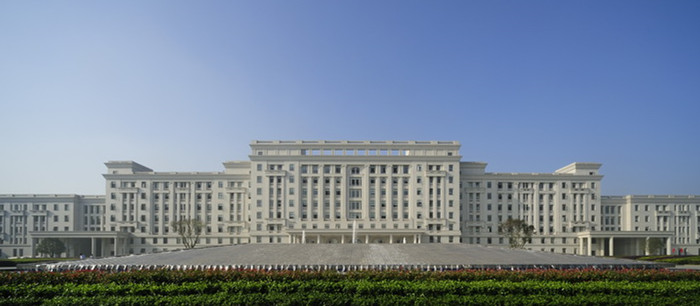
\includegraphics[width=0.55\textwidth]{main.jpg}}}
%\newsavebox\mybox
%\savebox\mybox{\tikz[color=red,opacity=0.3]\node{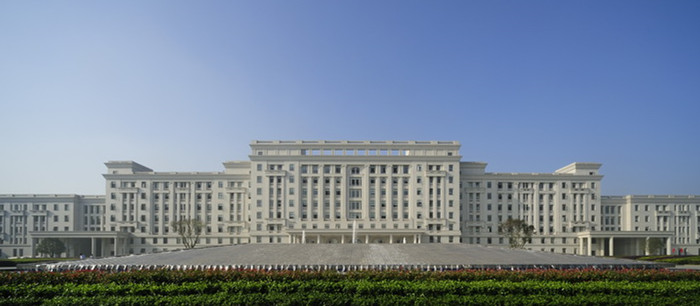
\includegraphics[width=0.55\textwidth]{main.jpg}};}
%\newwatermark*[allpages,angle=45,scale=6,xpos=-20,ypos=15]{\usebox\mybox}

%\node[opacity=.06]
\begin{document}

%----------------------------------------------------------------------------------------
%	FIRST PAGE HEADER
%----------------------------------------------------------------------------------------


\includegraphics[width=0.6\textwidth]{logo.png} % Logo

\vspace{-1em} % Pull the rule closer to the logo

\rule{\linewidth}{1pt} % Horizontal rule

\vspace{-4em} % Pull the address closer to the rule
%\bigskip\bigskip % Vertical whitespace

\hfill
\begin{FlushRight}
\begin{tabular}{l @{}}
	\textbf{University of Electronic Science and Technology of China} \\
	~~~~~~~~~~~~~~~~~No.2006, Xiyuan Ave, West Hi-Tech Zone, 611731, \\ 
	~~~~~~~~~~~~~~~~~~~~~~~~~~~~~~~~~~~~~~~~~~~~~~~~Chengdu, Sichuan, P. R. China \\
	~~~~~~~~~~~~~~~~~~~~~~~~~~~~~~~~~~~~~~~~~~~~~~~~~~~~~~~~http://www.uestc.edu.cn 
\end{tabular}
\end{FlushRight}

\today \bigskip\\ % Date
\vspace{-3em}
\begin{center}
 \textbf{\Large Letter of Recommendation}   
\end{center}


\begin{FlushLeft}
\textbf{To Whom It May Concern}
\end{FlushLeft}

\bigskip % Vertical whitespace

%----------------------------------------------------------------------------------------
%	ADDRESSEE AND GREETING
%----------------------------------------------------------------------------------------

%\begin{tabular}{@{} l}
%	Mrs.\ XXX \\
%	Recruitment Officer \\
%	The Corporation \\
%	123 Pleasant Lane \\
%	City, State 12345
%\end{tabular}

%\bigskip % Vertical whitespace

%Dear Mrs.\ XXX,

%\bigskip % Vertical whitespace

%----------------------------------------------------------------------------------------
%	LETTER CONTENT
%----------------------------------------------------------------------------------------

%\watermark{\centering\put(90,-450){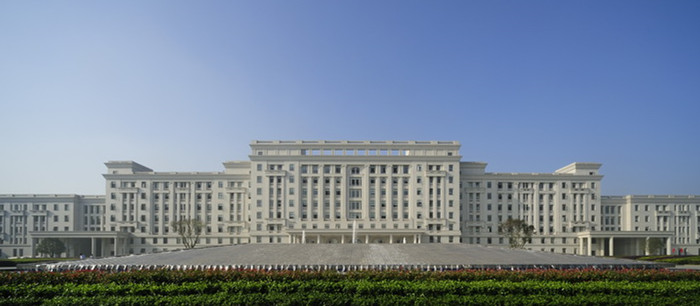
\includegraphics[width=0.7\textwidth]{main.jpg}}}
PARAGRAPH ONE: State the reason for the letter, name the position or type of work you are applying for and identify the source from which you learned of the opening (i.e. career development center, newspaper, employment service, personal contact).

PARAGRAPH TWO: Indicate why you are interested in the position, the company, its products, services - above all, stress what you can do for the employer. If you are a recent graduate, explain how your academic background makes you a qualified candidate for the position. If you have practical work experience, point out specific achievements or unique qualifications. Try not to repeat the same information the reader will find in the resume. Refer the reader to the enclosed resume or application which summarizes your qualifications, training, and experiences. The purpose of this section is to strengthen your resume by providing details which bring your experiences to life. 
 
PARAGRAPH THREE: Request a personal interview and indicate your flexibility as to the time and place. Repeat your phone number in the letter and offer assistance to help in a speedy response. For example, state that you will be in the city where the company is located on a certain date and would like to set up an interview. Alternatively, state that you will call on a certain date to set up an interview. End the letter by thanking the employer for taking time to consider your credentials. 

 
PARAGRAPH THREE: Request a personal interview and indicate your flexibility as to the time and place. Repeat your phone number in the letter and offer assistance to 

PARAGRAPH TWO: Indicate why you are interested in the position, the company, its products, services - above all, stress what you can do for the employer. If you are a recent graduate, explain how your academic background makes you a qualified candidate for the position. If you have practical work experience, point out specific achievements or unique qualifications. Try not to repeat the same information the reader will find in the resume. Refer the reader to the enclosed resume or application which summarizes your qualifications, training, and experiences. The purpose of this section is to strengthen your resume by providing details which bring your experiences to life. 
 


\bigskip % Vertical whitespace

Sincerely,

\vspace{30pt} % Vertical whitespace

Professor Green Stone\\
School of Computer Science and Engineering\\
University of Electronic Science and Technology of China\\
E-mail:stone@uestc.edu.cn~ \ Tel: +8613228106532


%\bigskip % Vertical whitespace
%\begin{FlushLeft}
%
\includegraphics[width=0.13\textwidth]{sign.jpg}\\ % Logo
%\end{FlushLeft}
%\vspace{-5pt} % Vertical whitespace
%\begin{FlushLeft}
%John Smith
%\end{FlushLeft}


\end{document}
